% Gas-padding ablation / mechanism attribution.
\subsection{Gas-Padding Ablation}
\label{sec:eval-ablation}

Only the gas measurements vary across policies within the selected feature set (Section~\ref{sec:eval-threat}).
We therefore use the ablation to assess how randomized gas padding affects the attackers' ability to infer hidden policy information.

We compare two configurations, B1 and B2, that differ only in whether randomized gas padding is enabled.
Both use the fixed circuit, commitment-only interface, and TPS execution profile.
We evaluate both configurations on the same policy subset, selected deterministically from the evaluation corpus.
B1 disables padding for both policy commitment and access transactions, whereas B2 enables it for both.
B2 uses the same protection configuration as the PCH, PI, and SPP evaluations (Sections~\ref{sec:eval-pch}, \ref{sec:eval-pi}, and~\ref{sec:eval-spp}).

To quantify the effect of padding on attack performance, we compare the absolute AUC deviation from $0.5$ under B1 and B2.
For each paired train/test split $s$, we define
%
\begin{equation}
	\Delta_{\text{leak},s} =
	|\mathrm{AUC}_{\mathrm{B1},s} - 0.5| -
	|\mathrm{AUC}_{\mathrm{B2},s} - 0.5|,
	\label{eq:delta-leak}
\end{equation}
%
where positive values mean padding moved the attacker closer to chance.

For each task, we compute $\Delta_{\text{leak},s}$ over $30$ paired train/test splits, one for each random seed, using the same test policies for B1 and B2 in each split.
We report the mean $\Delta_{\text{leak}}$ with a $95\%$ percentile-bootstrap confidence interval (CI), obtained by resampling the split-level differences.
Table~\ref{tab:ablation-gas-padding} summarizes the results, and Figure~\ref{fig:ablation-paired} visualizes the comparison between B1 and B2.

% Source of record (supervised rows + counts):
%   python/results/supervised_analysis/gas_padding_supervised_deltaLeakage.csv
%   (metadata: gas_padding_supervised_metadata.json)
% B1 = unpadded gas transcript; B2 = deployed randomized access-gas padding.
% Effect = |AUC_B1-0.5| - |AUC_B2-0.5|; 95% repeated-split stability interval over
% 30 paired seeds (nonContemporaneous B1/B2 profiles).
% This table is ILLUSTRATIVE: the four supervised rows are representative contrasts whose
% stability interval of dLeak excludes zero (genuine reduction). They are NOT the full set.
% The full per-contrast distribution (all 49 rf + 49 lr contrasts, colored by dLeak CI
% sign) is the primary evidence and lives in Fig. fig:ablation-paired. Full-set counts:
%   RF: 36 reduce / 13 no-eff / 0 neg;  LR: 36 reduce / 11 no-eff / 2 neg.
% The unsupervised-ARI and gas-cost rows below are retained from the deployed on-chain
% ablation run (experiments/ablation/gas_padding/...); they are not part of the Python
% supervised recompute.
\begin{table}[H]
  \centering
  \caption{Gas-padding ablation on Polygon Amoy: representative contrasts illustrating the
    padding effect. B1 (no gas padding) and B2 (deployed, randomized access-gas padding) are
    aligned on the same policy set. Supervised AUC is the random-forest score (the stronger
    of the two classifiers here; see Section~\ref{sec:eval-method}); clustering reports K-Means ARI.
    $\Delta_{\text{leak}}>0$ (defined in the text) means padding moved the attacker toward chance,
    reported as the mean with a $95\%$ stability interval over $30$ paired splits. Each supervised
    row is, per experiment, the largest-signal contrast whose $\Delta_{\text{leak}}$ interval excludes
    zero (two for SPP), chosen to avoid cherry-picking. The full per-contrast distribution is in
    Figure~\ref{fig:ablation-paired}.}
  \label{tab:ablation-gas-padding}
  \begin{tabular}{lp{0.34\linewidth}cc}
    \toprule
    Attack & Target & B1 (unpad.) & B2 (pad.) \\
    \midrule
    \multicolumn{4}{l}{\textbf{Supervised} (RF AUC; $\Delta_{\text{leak}}$ with $95\%$ interval)} \\
    SPP   & \texttt{nestingDepth flat/deep}   & $0.847$ & $0.553$ \\
          & \quad $\Delta_{\text{leak}}=0.280$ CI$[0.254,0.304]$ & & \\
    SPP   & \texttt{structureType trivial/negation\_heavy} & $0.843$ & $0.524$ \\
          & \quad $\Delta_{\text{leak}}=0.276$ CI$[0.248,0.301]$ & & \\
    PCH   & ICD ch8                          & $0.918$ & $0.410$ \\
          & \quad $\Delta_{\text{leak}}=0.327$ CI$[0.302,0.349]$ & & \\
    PI    & \texttt{semantic\_equivalent}\,$^{\dagger}$  & $0.361$ & $0.500$ \\
          & \quad $\Delta_{\text{leak}}=0.140$ CI$[0.084,0.205]$ & & \\
    \midrule
    \multicolumn{4}{l}{\textbf{Unsupervised} (K-Means ARI)} \\
    PCH   & ICD-10 chapter                   & $0.064$ & $-0.005$ \\
    SPP   & logic structure                  & $0.043$ & $-0.001$ \\
    SPP   & predicate count                  & $0.054$ & $0.001$  \\
    \midrule
    \multicolumn{4}{l}{\textbf{Gas cost} (mean, B1 $\to$ B2)} \\
    \multicolumn{2}{l}{Commit gas} & $216{,}562$ & $303{,}556$ ($+40.2\%$) \\
    \multicolumn{2}{l}{Access gas} & $546{,}876$ & $753{,}310$ ($+37.7\%$) \\
    \bottomrule
  \end{tabular}

  \noindent{\footnotesize{$^{\dagger}$ B1 sits below $0.5$: the unpadded attacker separates the
  pair in the inverted direction (still $0.14$ from chance). $\Delta_{\text{leak}}$ is defined on
  $|\mathrm{AUC}-0.5|$.}}
\end{table}


Figure~\ref{fig:ablation-paired} shows each supervised task as one point, giving $20$ PCH, $21$ SPP, and $4$ PI tasks per panel.
The horizontal and vertical axes give the absolute deviation from $0.5$ of the mean AUC over the $30$ splits under B1 and B2, respectively.
A mean AUC below $0.5$ therefore also counts as a deviation.
Points below the diagonal indicate that padding moves the mean AUC closer to chance.
Both panels show the same pattern. Tasks with large deviations under B1 move well below the diagonal, whereas tasks near chance under B1 stay in the lower-left corner on both sides of the diagonal.

For RF, $21$ tasks have mean AUCs that deviate from $0.5$ by more than $0.15$ under B1.
Under B2, all $21$ fall below this level, and their median deviation is $0.037$, comparable to $0.041$ for the remaining $24$ tasks.
The confidence intervals for $\Delta_{\text{leak}}$ lie entirely above zero for all $21$ tasks, supporting a reduction in deviation from chance.
Across all tasks, the median deviation decreases from $0.137$ under B1 to $0.038$ under B2.
LR shows a similar pattern.
All $19$ tasks with deviations above $0.15$ under B1 fall below this level under B2, and the median deviation across all tasks decreases from $0.111$ to $0.037$.



Tasks already close to chance under B1 show no consistent change after padding.
For RF, $12$ tasks have CIs for $\Delta_{\text{leak}}$ that include zero, and their B1 deviations are at most $0.095$.
Another $6$ tasks have CIs entirely below zero, indicating increased deviation from chance, although their B1 deviations are at most $0.045$.
The largest increase occurs for ch5, whose mean AUC changes from $0.455$ under B1 to $0.631$ under B2.
Such increases may reflect chance associations between the randomly drawn padding targets and the hidden labels.
Related diagnostic analyses for ch5 and the \texttt{nestingDepth} comparison \texttt{medium}/\texttt{deep} illustrate this effect (Sections~\ref{sec:eval-pch} and~\ref{sec:eval-spp}).

\begin{figure}[htbp]
	\centering
	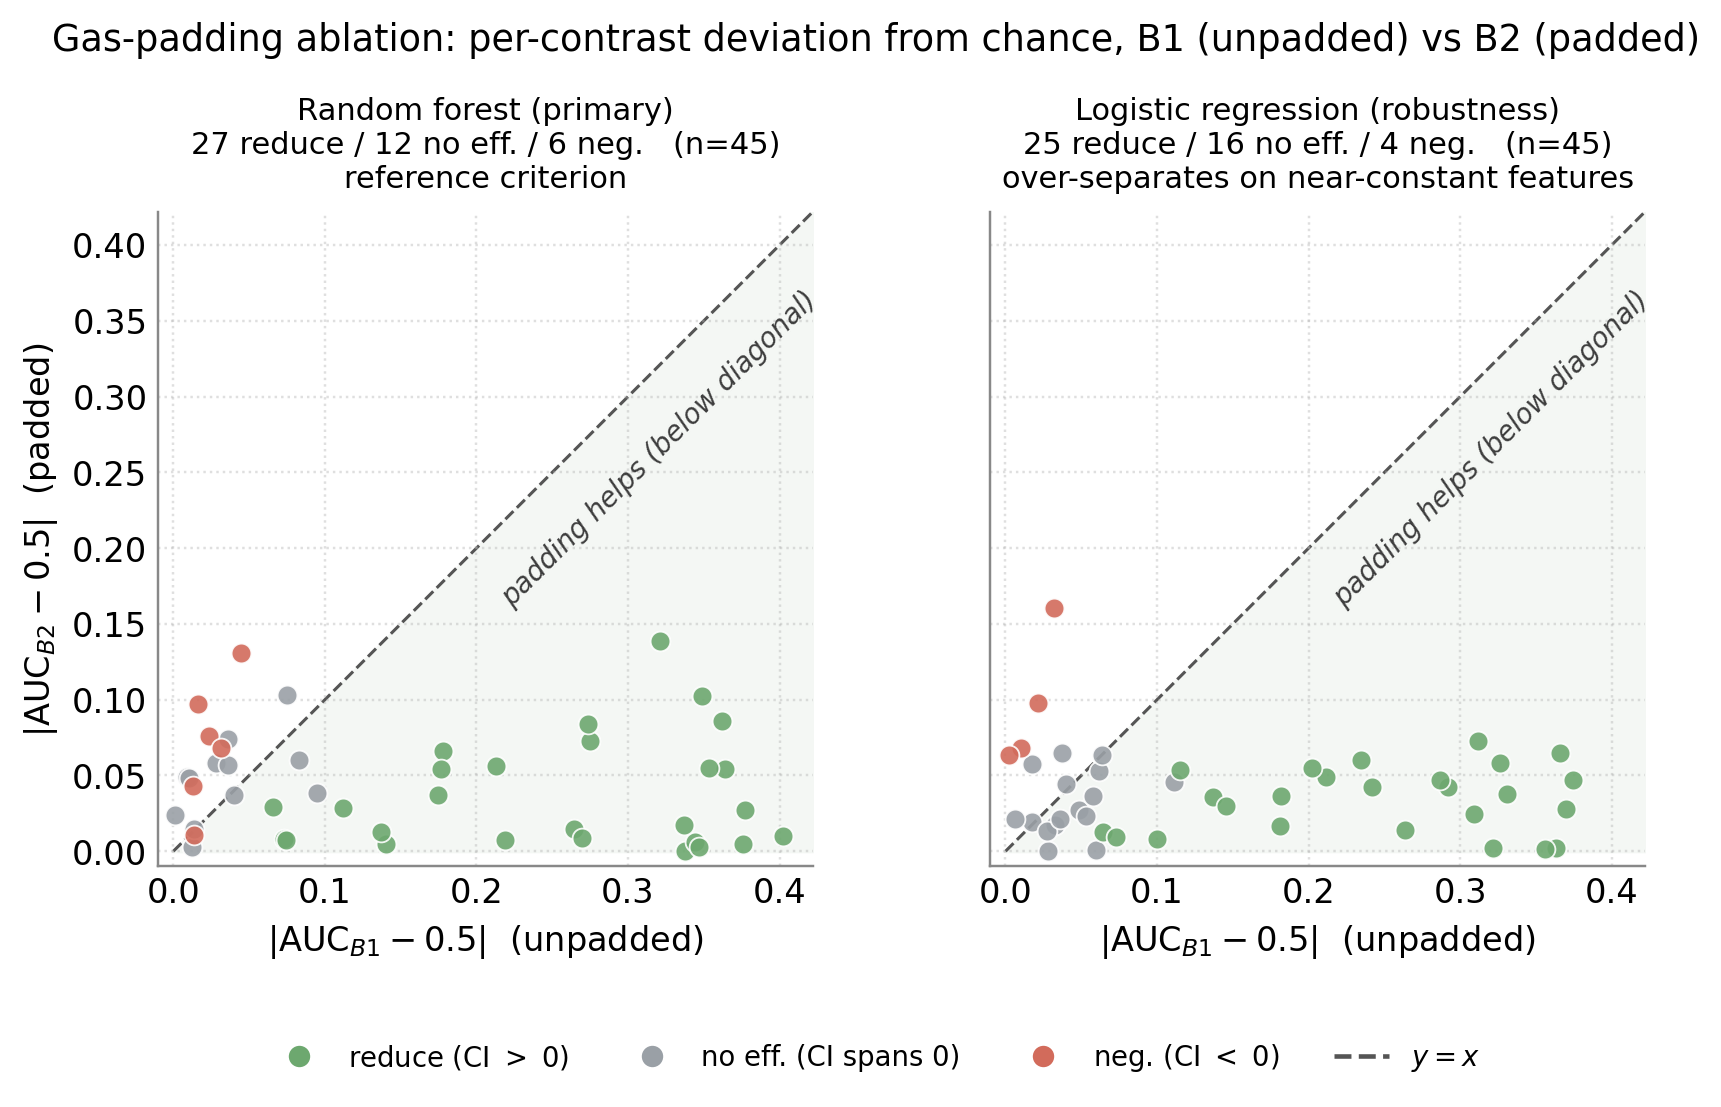
\includegraphics[width=\linewidth]{ablation_paired_scatter.png}
	\caption{Gas-padding ablation over the $45$ supervised tasks: (\textbf{a}) RF; (\textbf{b}) LR. Each point is one task, placed by the absolute deviation of its mean AUC from $0.5$ under B1 (horizontal axis) and B2 (vertical axis). Points below the dashed line $y=x$ moved closer to chance with padding. Blue, gray, and red points have $95\%$ CIs of $\Delta_{\text{leak}}$ above zero, spanning zero, and below zero, respectively.}
	\label{fig:ablation-paired}
\end{figure}

The clustering analysis provides complementary evidence.
Under B2, NMI decreases by $0.670$ for balanced PI pairs, $0.349$ for DUO terms, and $0.102$ for logical structure, with all three bootstrap confidence intervals excluding zero (Table~\ref{tab:ablation-gas-padding}).
With padding, NMI is at most $0.020$ for all three targets.

We next examine the source of the gas differences under B1.
Across the $1{,}119$ executions, unpadded access gas ranges from $723{,}288$ to $723{,}564$, excluding the first cold-start call.
Calldata analysis identifies two main sources of label-correlated variation arising from zero- and non-zero-byte pricing~\cite{akhunov2019eip2028}.
Different requester-pseudonym encodings produce an observed $192$-gas gap associated with profile-predicate use.
Sequential policy and resource identifiers introduce a further $24$-gas difference correlated with logical structure because policies were committed in groups by logical form.

Padding compensates for these calldata-pricing differences by bringing transaction gas consumption to the sampled target.
The remaining overhead varies by less than $100$ gas (Section~\ref{sec:eval-pch}), while the target varies by $\pm 105{,}000$ gas.
This provides a mechanism-level explanation for the reduced separability observed under B2.
